\documentclass[11pt,a4paper]{article}

% --- Paquetes de Idioma y Codificación ---
\usepackage[utf8]{inputenc}
\usepackage[T1]{fontenc}
\usepackage[spanish,es-tabla]{babel}

% --- Geometría de Página ---
\usepackage[top=2.2cm, bottom=2.2cm, left=2.2cm, right=2.2cm]{geometry}

% --- Tipografía y Párrafos ---
\usepackage{setspace}
\setstretch{1.08}
\usepackage{parskip}
\setlength{\parskip}{0.45em}
\setlength{\parindent}{0pt}

% --- Paquetes Matemáticos ---
\usepackage{amsmath,amssymb,amsfonts}

% --- Tablas Técnicas ---
\usepackage{booktabs}
\usepackage{tabularx}
\usepackage{array}
\usepackage{multirow}

% --- Gráficos y Figuras ---
\usepackage{graphicx}
\usepackage{float}
\usepackage{tikz}
\usetikzlibrary{shapes.geometric, arrows.meta, positioning, fit, backgrounds, calc}

% --- Listas ---
\usepackage{enumitem}
\setlist[itemize]{itemsep=0.2em, topsep=0.3em, parsep=0pt}
\setlist[enumerate]{itemsep=0.2em, topsep=0.3em, parsep=0pt}
\setlist[description]{itemsep=0.2em, topsep=0.3em, parsep=0pt}

% --- Encabezados y Pies de Página (Fancyhdr) ---
\usepackage{fancyhdr}
\pagestyle{fancy}
\fancyhf{}
\fancyhead[L]{\small\bfseries Universidad Nacional de La Plata (UNLP)}
\fancyhead[R]{\small\bfseries Trabajo Integrador Final - IoT 2026}
\fancyfoot[C]{\thepage}
\renewcommand{\headrulewidth}{0.4pt}
\renewcommand{\footrulewidth}{0pt}

% --- Títulos de Secciones ---
\usepackage{titlesec}
\titleformat{\section}{\normalfont\Large\bfseries}{\thesection}{1em}{}
\titlespacing*{\section}{0pt}{10pt}{4pt}
\titleformat{\subsection}{\normalfont\large\bfseries}{\thesubsection}{1em}{}
\titlespacing*{\subsection}{0pt}{8pt}{3pt}
\titleformat{\subsubsection}{\normalfont\normalsize\bfseries}{\thesubsubsection}{1em}{}
\titlespacing*{\subsubsection}{0pt}{6pt}{2pt}

% --- Enlaces y Referencias ---
\usepackage{hyperref}
\hypersetup{
    colorlinks=true,
    linkcolor=blue!65!black,
    urlcolor=blue!65!black,
    citecolor=blue!65!black
}


\begin{document}

% ==============================================================================
% ENCABEZADO Y TÍTULO COMPACTO (Máximo media carilla según especificación)
% ==============================================================================
\begin{center}
    {\bfseries\large UNIVERSIDAD NACIONAL DE LA PLATA} \\[0.1cm]
    {\bfseries\normalsize FACULTAD DE INFORMÁTICA --- INTERNET DE LAS COSAS 2026} \\[0.3cm]
    \rule{\textwidth}{0.8pt} \\[0.25cm]
    \vspace{0.2cm}
    {\bfseries\LARGE Sistema de Geofencing para Ganado con Enlace LoRa de Bajo Consumo y Alertas} \\[0.2cm]
    \rule{\textwidth}{0.4pt} \\[0.25cm]
    {\bfseries Autores:} Cid De La Paz, Alejo --- Pacchialat, Taciano \\[0.3cm]
\end{center}

\begin{abstract}
\noindent El presente informe técnico describe el diseño, arquitectura e implementación de una plataforma de monitoreo de ubicación y delimitación perimetral virtual (geofencing) para ganado bovino en entornos rurales sin cobertura de telefonía celular. El sistema articula nodos móviles de borde (collares) basados en microcontroladores ESP32 con receptores GPS y transceptores LoRa SX1278 a 433~MHz operando bajo ciclos estrictos de temporización en \textit{Deep Sleep}. Los paquetes de telemetría son capturados por una compuerta de enlace (\textit{Gateway}) ESP32-CAM y retransmitidos vía MQTT e InfluxDB hacia un servidor local Node-RED y contenedores Docker. La verificación espacial punto-en-polígono (\textit{Ray-Casting}) y el control paramétrico se gestionan desde una interfaz de monitoreo y un bot bidireccional de Telegram con alertas proactivas.
\end{abstract}

\vspace{0.2cm}
\rule{\textwidth}{0.4pt}
\vspace{0.2cm}

% ==============================================================================
% SECCIONES MODULARES (\input)
% ==============================================================================
\section{Introducción y Objetivos}

La gestión y localización de ganado bovino en extensiones rurales extensas presenta restricciones operativas críticas vinculadas a la ausencia de infraestructura eléctrica y de cobertura de telefonía celular comercial. Los sistemas tradicionales de delimitación física con alambrado perimetral o boyeros eléctricos incurren en elevados costos de mantenimiento e imposibilitan la modificación dinámica del área de pastoreo.

El presente proyecto implementa una plataforma de delimitación geográfica virtual por software (\textit{geofencing}) integrada con telemetría de posicionamiento por satélite y un enlace de comunicación \textit{LoRa}. El sistema permite monitorear las coordenadas de cada animal y generar alertas ante salidas perimetrales o fallas de conectividad, operando de forma autónoma sin depender de redes de terceros en el campo.

\subsection{Objetivos del Sistema}
\begin{description}
    \item[Desarrollo de nodo de borde de bajo consumo:] Diseñar un collar móvil autónomo basado en el microcontrolador ESP32 con receptor GPS simulado y transceptor LoRa SX1278 (433~MHz), operando bajo ciclos temporizados en modo \textit{Deep Sleep} para maximizar la vida útil de la batería.
    \item[Enrutamiento local:] Implementar un nodo de \textit{Gateway} capaz de capturar paquetes de LoRa e inyectarlos a una red Wi-Fi local mediante el protocolo MQTT.
    \item[Procesamiento espacial:] El cálculo algebraico del perímetro se realiza en el microcontrolador del collar, ejecutando el algoritmo de pertenencia poligonal, que luego se sincroniza con un servidor central local (Node-RED) con acceso a almacenamiento histórico y temporal de InfluxDB.
    \item[Control remoto:] Proveer una interfaz web interactiva con representación en mapa para visualización de telemetría y edición paramétrica de límites del Geofence, complementada con un bot bidireccional de Telegram para alertas e interrogación de estado.
\end{description}

\section{Arquitectura General y Selección de Hardware}

La topología del sistema adopta una estructura jerárquica de tres capas: capa de borde (collares móviles en el ganado), capa de agregación (Gateway LoRa/Wi-Fi), y capa de backend (servidor local con contenedores Docker).

\subsection{Diagrama de Bloques del Sistema}

La Figura~\ref{fig:arch_global} detalla la interconexión de componentes de hardware y los protocolos de comunicación utilizados en cada tramo del flujo de datos.

\begin{figure}[H]
\centering
\begin{tikzpicture}[
    node distance=1.1cm and 1.4cm,
    block/.style={rectangle, draw=black, thick, fill=gray!8, text width=3.1cm, align=center, minimum height=1.3cm, font=\small},
    cloud/.style={rectangle, rounded corners=4pt, draw=black, thick, fill=blue!5, text width=3.4cm, align=center, minimum height=1.3cm, font=\small},
    server/.style={rectangle, draw=black, thick, fill=green!5, text width=3.3cm, align=center, minimum height=1.3cm, font=\small},
    arrow/.style={-{Stealth[scale=1.1]}, thick}
]
    % Nodos
    \node[block] (edge) {\textbf{Módulo Edge (Collar)}\\ESP32 + GPS Neo-6M\\+ Radio SX1278};
    \node[block, right=of edge] (gateway) {\textbf{Módulo Gateway}\\ESP32-CAM\\+ Radio SX1278};
    \node[cloud, right=of gateway] (broker) {\textbf{Broker MQTT}\\Mosquitto (Docker)\\\footnotesize\texttt{geofence/heartbeat}};
    
    \node[server, below=0.7cm of broker] (nodered) {\textbf{Motor de Reglas}\\Node-RED (Docker)\\Ray-Casting \& Alertas};
    \node[server, left=of nodered] (influx) {\textbf{Base de Datos}\\InfluxDB 1.8\\\footnotesize\texttt{geofence\_config}};
    \node[server, below=0.7cm of nodered] (ui) {\textbf{Interfaz Web \& Bot}\\Dashboard HUD / Telegram\\Control Bidireccional};

    % Conexiones
    \draw[arrow] (edge) -- node[above, font=\footnotesize] {LoRa 433~MHz} node[below, font=\footnotesize] {OOK/FSK/LoRa} (gateway);
    \draw[arrow] (gateway) -- node[above, font=\footnotesize] {Wi-Fi / TCP} node[below, font=\footnotesize] {MQTT Pub} (broker);
    \draw[arrow] (broker) -- node[right, font=\footnotesize] {Sub / Inyecta TS} (nodered);
    \draw[arrow] (nodered) -- node[above, font=\footnotesize] {Consulta/Guarda} (influx);
    \draw[arrow] (nodered) -- node[right, font=\footnotesize] {Alertas / API REST} (ui);
    \draw[arrow, dashed] (ui) -| node[pos=0.25, below, font=\footnotesize] {POST \texttt{/api/update-fence}} (influx);

\end{tikzpicture}
\caption{Topología general del sistema de geofencing ganadero y flujo de información entre capas.}
\label{fig:arch_global}
\end{figure}

\subsection{Especificaciones Técnicas del Hardware}

Para satisfacer las restricciones de consumo en el collar y las exigencias de conectividad, se seleccionaron dos variantes del microcontrolador ESP32 de Espressif Systems combinadas con transceptores de radiofrecuencia. La Tabla~\ref{tab:hardware_specs} sistematiza las especificaciones operativas y la justificación de diseño para cada componente.

\begin{table}[H]
\centering
\small
\begin{tabularx}{\textwidth}{@{}l l l X@{}}
\toprule
\textbf{Componente} & \textbf{Modelo / IC} & \textbf{Especificación Principal} & \textbf{Función en el Sistema} \\ \midrule
\textbf{MCU Borde} & ESP32-WROOM-32D & Dual-core Xtensa LX6, 240~MHz & Procesamiento en collar, temporización con reloj de tiempo real (RTC) en Deep Sleep. \\ \addlinespace
\textbf{MCU Gateway} & ESP32-WROOM-32D & Dual-core Xtensa LX6, 240~MHz & Receptor base de interrupciones de radio e interfaz Wi-Fi hacia el servidor local. \\ \addlinespace
\textbf{Radio LoRa} & SX1278 & Frecuencia 433~MHz & Enlace RF de largo alcance ($>4$~km en línea de vista) con modulaciones de espectro ensanchado. \\ \addlinespace
\textbf{Receptor GPS} & Simulado & Mediante comandos UART al MCU & Adquisición de longitud y latitud. \\ \bottomrule
\end{tabularx}
\caption{Especificaciones y asignación de hardware del sistema.}
\label{tab:hardware_specs}
\end{table}

El enlace de radiofrecuencia opera en la banda ISM de 433~MHz con modulación LoRa. Esto garantiza un balance entre inmunidad al ruido electromagnético en zonas abiertas, velocidad de transmisión y tiempo en el aire, reduciendo el consumo energético en cada ráfaga de telemetría.

\section{Desarrollo y Arquitectura del Firmware}

El firmware del sistema de geofencing está estructurado en dos proyectos independientes desarrollados en C++ bajo el framework de Espressif (\textit{ESP-IDF}): el módulo móvil de borde (\texttt{edge-module}) incrustado en el collar del ganado y el módulo base de enlace (\texttt{gateway-module}). La arquitectura de ambos nodos prioriza la estabilidad de ejecución continua y el manejo eficiente de recursos temporales y de memoria.

\subsection{Módulo Edge}

El collar opera bajo restricciones energéticas. Para maximizar su autonomía sin perder capacidad de respuesta o trazabilidad espacial, el firmware implementa una máquina de estados temporizada regida por el controlador del Reloj de Tiempo Real (RTC) del ESP32. En el prototipo se alimentó al MCU mediante USB hacia la computadora, pero se realizó con la intención de tener una gran autonomía si fuera alimentado con baterías.


Durante la mayor parte de su ciclo operativo, el microcontrolador permanece en estado de bajo consumo profundo (\textit{Deep Sleep}), donde se desenergizan los núcleos de CPU, el controlador de radio LoRa y los periféricos estándar, reduciendo el consumo total a ($\mu$A). Para mantener la coherencia de telemetría entre ciclos de sueño sin acceder al almacenamiento no volátil Flash (lo que incrementaría el consumo y desgastaría el medio), las variables de control y contadores de secuencia se almacenan en la memoria estática lenta del RTC (\texttt{RTC\_DATA\_ATTR}). En este dominio de memoria persisten el contador incremental de despertares (\texttt{boot\_count}), las últimas coordenadas validadas y el estado actual de alarma del cerco.


El temporizador del RTC activa el sistema periódicamente cada 30~segundos. La Figura~\ref{fig:edge_states} ilustra el flujo secuencial de tareas ejecutado en cada ciclo de \textit{Wakeup}.

\begin{figure}[H]
\centering
\begin{tikzpicture}[
    node distance=1.1cm and 2.5cm,
    state/.style={rectangle, rounded corners=6pt, draw=black, thick, fill=gray!8, text width=3.3cm, align=center, minimum height=1.2cm, font=\footnotesize\bfseries},
    sleep/.style={rectangle, rounded corners=6pt, draw=black, thick, fill=blue!8, text width=3.3cm, align=center, minimum height=1.2cm, font=\footnotesize\bfseries},
    arrow/.style={-{Stealth[scale=1.0]}, thick}
]
    \node[sleep] (deepsleep) {Deep Sleep};
    \node[state, right=of deepsleep] (wakeup) {Despertar por RTC};
    \node[state, right=of wakeup] (gps) {Adquisición GPS \\(Simulado)};
    
    \node[state, below=0.9cm of gps] (tx) {Transmisión LoRa};
    \node[state, left=of tx] (rx) {Ventana Escucha LoRa (2~s)};
    \node[state, left=of rx] (downlink) {Procesar Downlink};

    \draw[arrow] (deepsleep) -- node[above, font=\scriptsize] {Timer RTC} (wakeup);
    \draw[arrow] (wakeup) -- (gps);
    \draw[arrow] (gps) -- node[right, font=\scriptsize] {} (tx);
    \draw[arrow] (tx) -- node[above, font=\scriptsize] {Abre Ventana} (rx);
    \draw[arrow] (rx) -- node[above, font=\scriptsize] {Trama RX OK} (downlink);
    \draw[arrow] (downlink) -- node[left, font=\scriptsize] {Ajusta Estado} (deepsleep);
    \draw[arrow] (rx) -- node[pos=0.3, right, font=\scriptsize] {Timeout 2s} (deepsleep);

\end{tikzpicture}
\caption{Diagrama de estados del módulo de borde.}
\label{fig:edge_states}
\end{figure}

Al salir de \textit{Deep Sleep}, la secuencia operativa se desarrollade la siguiente manera:
\begin{enumerate}
    \item \textbf{Inicialización:} El procesador verifica la causa de activación del RTC y recupera las variables de estado desde el registro \texttt{RTC\_DATA\_ATTR}.
    \item \textbf{Adquisición:} Se habilita la interfaz UART para capturar las coordenadas simuladas. Si el módulo obtiene una solución de posición válida, extrae la longitud y latitud. Si se agota el tiempo máximo de espera sin fijación, el sistema utiliza la última coordenada conocida y marca un indicador de telemetría degradada.
    \item \textbf{Transmisión:} El procesador empaqueta los datos posicionales, el indicador de batería, el contador de secuencias y el estado local en una estructura y ordena su emisión a través del bus SPI hacia el transceptor LoRa SX1278.
    \item \textbf{Ventana de recepción:} Tras finalizar la transmisión del paquete, el transceptor conmuta inmediatamente a modo recepción durante una ventana temporal estricta de $2000$~milisegundos ($2.0$~segundos). Esta ventana sincronizada permite que el Gateway transmita actualizaciones de parámetros del cerco sin obligar al collar a mantener el receptor encendido de forma permanente. Si el transceptor detecta un paquete entrante válida durante la ventana, la lógica interpreta el comando. Si la orden instruye una alarma perimetral, se envía en el próximo ciclo las nuevas coordenadas y el estado de FUERA.
    \item \textbf{Retorno:} Concluida la ventana de recepción y ejecutada la actuación local, el microcontrolador reconfigura el temporizador de alarma del RTC y desenergiza todos los buses, retornando al modo \textit{Deep Sleep}.
\end{enumerate}

\subsection{Módulo Gateway}

El módulo Gateway  opera de forma estacionaria y alimentado de forma continua. Su responsabilidad consiste en escuchar permanentemente el canal LoRa, recibir las ráfagas de telemetría entrantes, formatear las tramas en objetos JSON estructurados y publicarlos a través de Wi-Fi hacia el broker MQTT.

El transceptor SX1278 notifica la llegada de un paquete completo activando la línea digital de interrupción externa \texttt{DIO0}. Para garantizar ejecución la ISR se restringe estrictamente a la memoria interna RAM del procesador mediante el atributo de compilador \texttt{IRAM\_ATTR}, prohibiendo accesos indirectos a la memoria Flash externa que podrían generar demoras por fallas de caché. La ISR se limita a limpiar el flag de interrupción del hardware del radio y emitir una notificación directa hacia una tarea dedicada de FreeRTOS de alta prioridad.


El planificador del FreeRTOS desbloquea de inmediato la tarea manejadora de recepción LoRa al recibir la señal de la ISR. Esta tarea dedicada realiza la lectura de los registros del transceptor vía SPI, extrae la carga útil del paquete y deposita la estructura resultante en una cola de mensajes segura para concurrencia.

De forma concurrente, una segunda tarea de comunicación de red extrae los paquetes del búfer, los serializa y los transmite mediante MQTT hacia el broker.

\section{Backend}

El procesamiento de servidor y el almacenamiento de datos operan sobre un ecosistema de microservicios contenidos mediante Docker en un servidor local. 

\subsection{Stack Docker}

El servidor ejecuta cuatro contenedores interconectados en una red virtual privada aislada:
\begin{description}
    \item[Broker Mosquitto:] Actúa como concentrador MQTT local recibiendo las publicaciones del Gateway en el tópico \texttt{geofence/heartbeat} y notificando cambios perimetrales en \texttt{geofence/config\_update}.
    \item[Base de Datos InfluxDB:] almacena las posiciones históricas en la medición \texttt{cattle\_position} y la configuración del perímetro en \texttt{geofence\_config}.
    \item[Flujos Node-RED:] enrutamiento de paquetes, decodificación JSON, validación espacial de la geofence y exposición de endpoints.
\end{description}


\subsection{APIs}

La configuración del cerco virtual se almacena de manera persistente dentro de la medición \texttt{geofence\-\_config} de InfluxDB, conservando el cerco activo ante reinicios del servidor o de los servicios de Docker. La Tabla~\ref{tab:api_rest} detalla las especificaciones técnicas de los puntos de entrada expuestos por Node-RED y enrutados a través de Nginx.

\begin{table}[H]
\centering
\footnotesize
\begin{tabularx}{\textwidth}{@{}l l >{\raggedright\arraybackslash}p{3.8cm} >{\raggedright\arraybackslash}X@{}}
\toprule
\textbf{Método} & \textbf{Ruta (\texttt{/api/})} & \textbf{Carga Útil (Payload)} & \textbf{Comportamiento Técnico y Persistencia} \\ \midrule
\textbf{GET} & \texttt{fence/current} & \textit{Ninguno} & Consulta el último registro en \texttt{geofence\_config} de InfluxDB. Retorna objeto con \texttt{vertices} JSON y coordenadas del bounding box. Si no hay datos, emite polígono por defecto. \\ \addlinespace
\textbf{POST} & \texttt{update-fence} & JSON: \newline \texttt{\{vertices: [\{lat, lng\}]\}} & Valida arreglo de coordenadas, calcula límites geográficos mínimos y máximos (\texttt{min/max lat/lon}), inserta nuevo punto en \texttt{geofence\_config} y publica notificación en tópico MQTT \texttt{geofence/config\_update}. \\ \addlinespace
\textbf{POST} & \texttt{fence} & JSON: \newline \texttt{\{vertices: [\{lat, lng\}]\}} & Endpoint de compatibilidad directa con las vistas de edición web, enrutado al manejador transaccional de \texttt{update-fence}. \\ \bottomrule
\end{tabularx}
\caption{Especificación APIs.}
\label{tab:api_rest}
\end{table}


\section{Interfaz de Usuario}

La interacción del operador con el sistema se realiza a través de dos canales: un dashboard y bot de Telegram. Ambas interfaces operan sobre flujos de datos asincrónicos.

\subsection{Dashboard}

El tablero de control web funciona como una aplicación de página única, estructurada sobre primitivas de HTML5, JavaScript moderno (ES6+) y CSS nativo sin dependencias pesadas.

La representación gráfica del terreno y de las unidades ganaderas se ejecuta mediante la biblioteca de \textit{Leaflet.js}. Al iniciar la sesión, el cliente realiza una petición HTTP inicial hacia el endpoint \texttt{GET /api/fence/current} para obtenerj el cerco activo de la base de datos y trazar el polígono delimitador sobre la capa del mapa.

De manera paralela, la aplicación establece un canal de comunicación dúplex persistente mediante \textit{WebSocket} contra el motor Node-RED. Cada vez que el Gateway ingesta un nuevo paquete de telemetría por radio LoRa, el servidor retransmite el evento \texttt{update\_location} a los clientes web conectados. La lógica del frontend actualiza de inmediato las coordenadas del marcador correspondiente al animal, la información del enlace, el nivel de voltaje de la batería y la última marca de tiempo de sincronización.

Para permitir un ajuste de los límites del perímetro virtual sobre el terreno, la interfaz incorpora un panel lateral interactivo de vértices que habilita la modificación de la geocerca mediante eventos de teclado.

Al finalizar el ajuste, el operador acciona el comando de guardado, lo que desencadena la emisión de una petición \texttt{POST /api/update-fence}. El servidor recibe la nueva geometría, recalcula la caja (\textit{Bounding Box}) y actualiza en milisegundos las reglas de validación en todos los nodos de monitoreo activos, tal como se ilustra en la Figura~\ref{fig:dashboard_web}.

\begin{figure}[H]
    \centering
    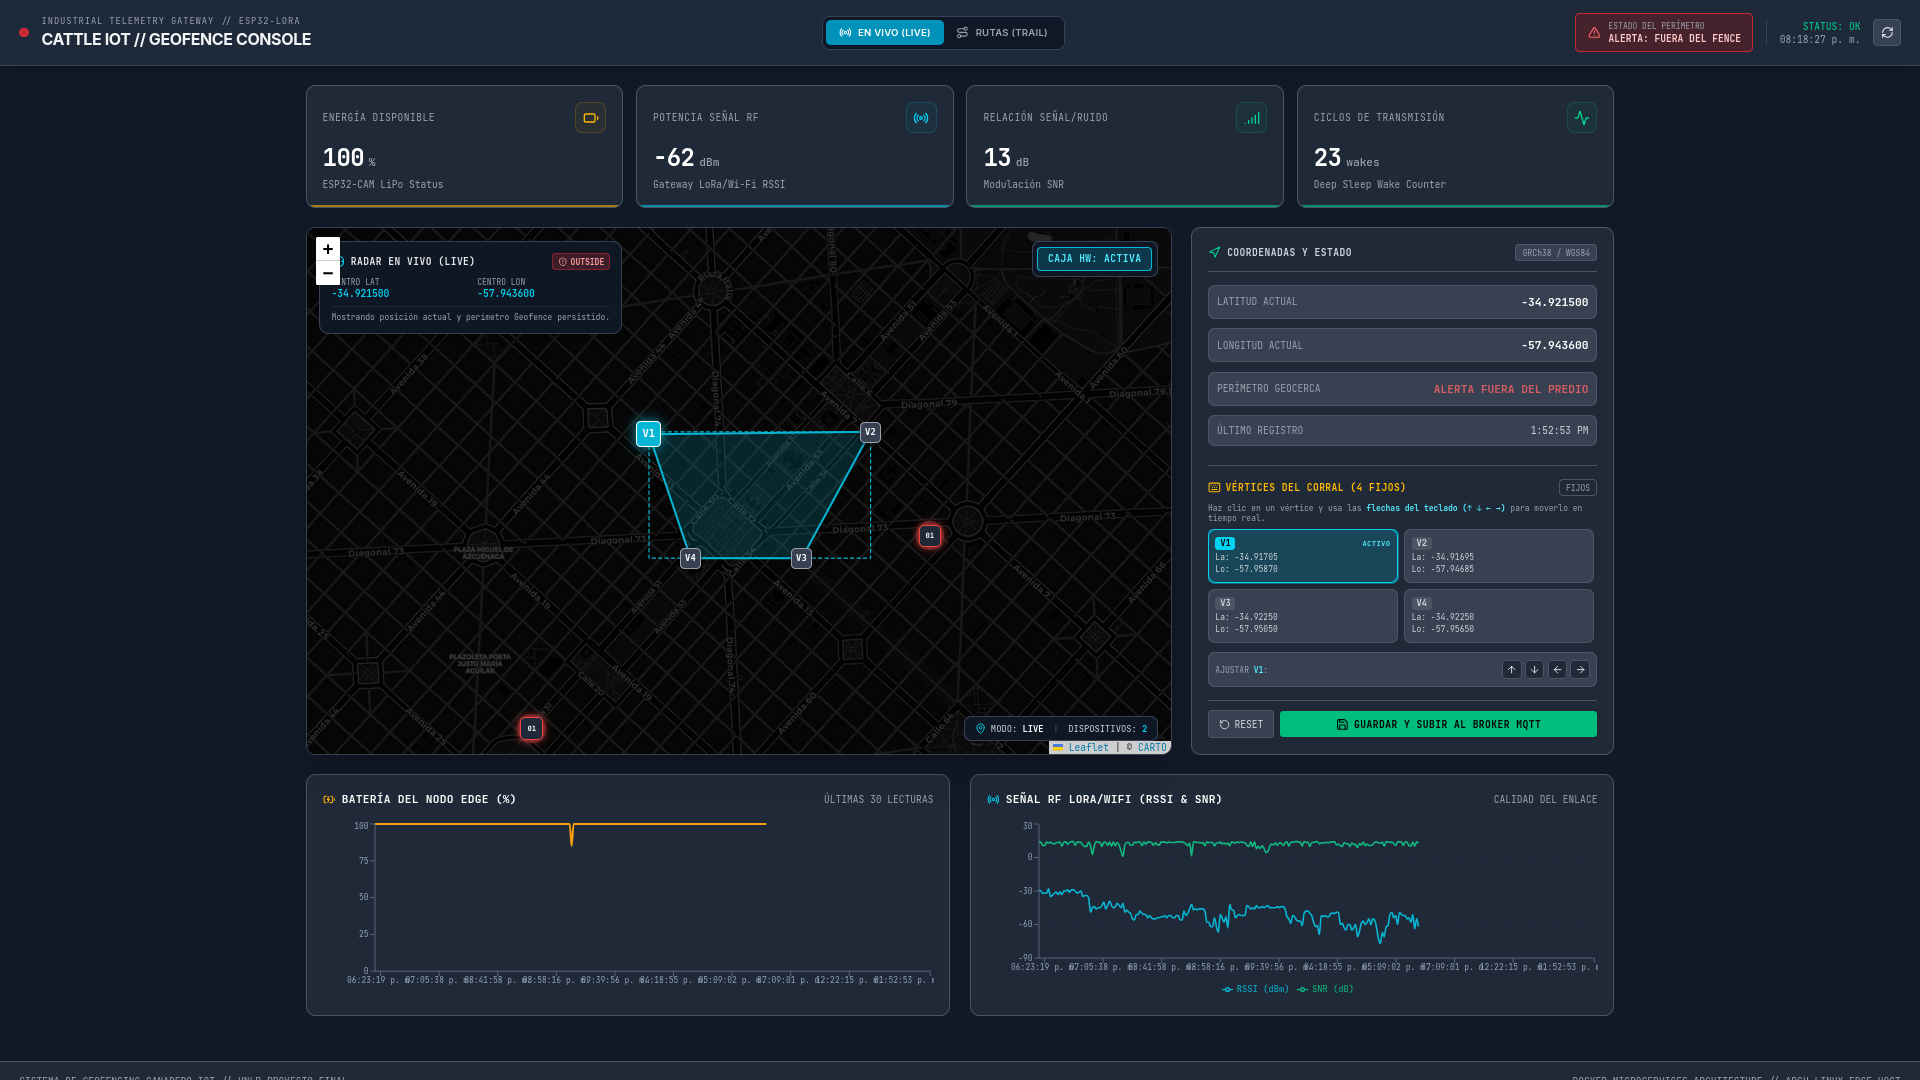
\includegraphics[width=0.98\textwidth]{secciones/image.png}
    \caption{Captura de pantalla del Dashboard.}
    \label{fig:dashboard_web}
\end{figure}

\subsection{Bot de Telegram}

La supervisión remota requiere un mecanismo de notificación push que no dependa de mantener un navegador web abierto continuamente. Para ello, el backend integra un bot de Telegram gestionado por la biblioteca \texttt{node-telegram-bot-api} dentro del entorno de Node-RED.

Cuando el algoritmo determina que la posición censada de un animal sale del cerco (\texttt{inside === false}), el módulo de notificaciones consulta en InfluxDB las últimas coordenadas reportadas del identificador del collar y estructura un mensaje de advertencia hacia los operadores.

El bot de Telegram opera como terminal de comandos remota, permitiendo al administrador del sistema intervenir de manera directa sobre los actuadores físicos del collar sin necesidad de acceder a la consola de servidor o al tablero web.


\section{Conclusiones y Trabajo Futuro}

El desarrollo y validación de este sistema demostró la viabilidad técnica de implementar monitoreo geoespacial sin cobertura celular. La arquitectura dividida en tres capas permitió aislar las restricciones energéticas del collar (Módulo Edge) mediante un enlace de radiofrecuencia LoRa en 433~MHz hacia un Módulo Gateway, el cual procesa y deriva la telemetría a una infraestructura centralizada basada en Docker, Node-RED e InfluxDB.

Desde la perspectiva algorítmica y de firmware, se resolvieron problemas críticos de concurrencia y consumo. El uso de la memoria estática del reloj de tiempo real \texttt{RTC\_DATA\_ATTR} conservó el contexto de operación durante los ciclos de \textit{Deep Sleep}. Asimismo, la inyección de marcas de tiempo en el servidor y la optimización por\textit{Bounding Box} en el cálculo de del posicionamiento en la cerca aseguraron una detección de fugas certera.


\end{document}
